%%!TEX TS-program = latex
\documentclass[12pt,letterpaper]{article}
\usepackage{epsfig}                 
\usepackage[authoryear]{natbib}
\usepackage{graphicx}
\usepackage{amsmath}
\usepackage{psfrag}
\usepackage{mathabx}
\renewcommand{\baselinestretch}{1.6}
\large
\pagenumbering{arabic}
\usepackage[usenames,dvipsnames]{color}
\usepackage{fullpage}
\bibliographystyle{genetics}
\usepackage{multirow}
\newcommand{\ye}{\hat{y}}
\newcommand{\xe}{\hat{x}}
\usepackage{color}
\usepackage[normalem]{ulem}  
	\newcommand{\gc}[1]{{ \color{red} #1}}
	\newcommand{\yb}[1]{{ \color{blue} #1}}




%Why do animals allow male control of female meiosis?
%Why does female meiosis allow the opportunity for exploitation by selfish sperm?
%sperm and egg genomes both favour the peaceful resolution of female meiotic drive
%strange bed fellows

%\title{Why does female meiosis allow the opportunity for exploitation by selfish sperm? BETTER TITLE?}
\title{Co-operation between the sexes trumps selfish control of female
  meiotic drive. Or 
Sperm do not evolve to collaborate in female meiotic drive. Or Why does female meiosis allow the opportunity for exploitation by selfish sperm? }

\author{Yaniv Brandvain \\ email: ybrandvain@gmail.com  \and Graham Coop \\ email: gmcoop@ucdavis.edu }

\usepackage{fancyhdr}
\pagestyle{fancy}
\lhead{}
\rhead{}
\renewcommand{\headrulewidth}{0.0pt}
\rfoot{}
\cfoot{\thepage}
\date{}
\bibliographystyle{plain}
\begin{document}
\maketitle
\begin{center}
Center for Population Biology \& Department of Evolution and Ecology \\ University of California - Davis \\ Davis, CA, 95616
\end{center}

%FIgures 
{\bf Abstract:}
\newpage

\section*{Introduction}

Despite the apparent unity of the organism, alleles can
gain an evolutionary advantage at a cost to  individual fitness
\citep{Burt2006}, often by exploiting meiosis and gametogenesis.
Because only one of the four products of female meiosis is transmitted to the egg, female meiosis is particularly vulnerable to such exploitation \citep{Sandler1957,Pardo-ManuelDeVillena2001a}. 
An allele that biases female meiosis in its favor (i.e. a meiotic driver), may increase in frequency even if this driver entails a pleiotropic fitness cost \citep{Prout1973}, generating a genetic conflict between the success of the driver and organismal fitness.
Meiotic drivers observed in nature (in both plants
\citep{Buckler1999,Fishman2005,Fishman2008}, and animals
\citep{Agulnik1990,Wu2005,Pardo-ManuelDeVillena2001c}) highlight this
conflict -- the selfish benefits of drive and the associated
pleiotropic fitness costs sustain a balanced polymorphism
\citep{Prout1973}, 
and often generate an ongoing evolutionary escalation of drive suppressors and enhancers \citep{Dawe1996,Fishman2008}. 
The threat of meiotic drive to organismal fitness is potentially so
severe that many basic properties of
meiosis and o\"{o}genesis, including the initial genome doubling in
meiosis I \citep{Haig1991}, arrested female meiosis
\citep{Mira1998}, centromere machinery \citep{MalikHenikoff}, and sex differences in the recombination rate \citep{Haig2010,Brandvain2012} 
have perhaps evolved to disrupt meiotic drive and enforce fairness. 

It is therefore somewhat surprising that despite the intense evolutionary pressure on female meiosis to prevent meiotic drive, 
it is potentially open to sabotage by a virtual stranger -- a haploid sperm genome.
That is, in many animal species, female meiosis is competed only after fertilization \citep{Masui_book}, 
creating ample opportunity for interaction between the sperm and female meiotic machinery. 
For example, an allele in sperm that facilitates meiotic drive by a genetically equivalent allele in female meiosis %(a  heteromorphic dyad), 
     could presumably rapidly spread through the population. 
At first sight, it seems as although female meiosis is primed to be exploited by selfish sperm systems.  
Why then is the requirement of fertilization to complete female meiosis so ubiquitous? 

It is certainly not the case that animals are mechanistically incapable of circumventing this requirement.
The stage at which female meiosis requires fertilization varies widely across taxa, and in a few animal taxa, 
	female meiosis is complete upon ovulation (that is fertilization is not required for female meiosis \citep[see
	Table 1 of ][]{Masui_book}). 

It is also not the case that sperm is mechanistically incapable of influencing the outcome of female meiosis.
Mechanistic evidence for this possibility comes from
\emph{C. elegans} the fact that premature deployment of the aster (a vital component of mitotic
machinery) provided by the sperm can disrupting MII meiotic segregation
in the egg, leading to a triploid zygote \citep{McNally2012}. 
Additionally, genetic evidence suggests that the transmission patterns
in heterozygous females many potentially depend on sperm haplotype. 
Specifically, two female meiotic drive systems in mouse (In and Om), both operate by distorting the second meiotic division, 
and in both systems the outcome of female meiosis depends the genotype of the fertilizing sperm \citep{Agulnik1993,Wu2005}. 
While such genetic evidence is suggestive, we note the difficulty in
ruling out the alternative hypothesis of early selection on zygotes \citep[pages
52-54][]{Burt2006}.

%However,  we acknowledge the difficulty in ruling out early mortality
%as an alternative explanation of the 
%specifics of these putative drivers \citep[Give page numbers to
%discussion of this in][]{Burt2006}. \gc{should be careful here as the
 % Om locus is pretty convincingly a meiotic driver, doubts have just
 % been raised about whether IN is. Whether the sperm dep nature of
 % either is robust to this is I think more at question.}


Here, we develop population genetic models exploring the evolution of sperm influence on female meiotic drive. 
%In this article we explore through simple population genetic models the consequences of alleles that influence the outcome of female meiosis.
These models show that sperm modifiers of female meiotic drive are
unlikely to create a sustained conflict, and therefore 
female meiosis will have little incentive to evolve resistance to them.
In fact, the interests of sperm and egg  genomes' are often aligned, as both are invested in the fate of the resultant zygote (as was speculated for the In locus \citep{Pomiankowski1993}).
Therefore, there is little selective benefit to females in preventing sperm to influence female meioses,
	indeed features of meiosis may evolve that facilitate the interaction of sperm with female meiosis. 

\section*{Results}

\subsection*{ Invasion of the population by a driving allele that promotes
itself.}
%%%%%%%%%%%%%%%%%%%%%%%%%
% PLEIOTROPY MODEL [self-promoting]
%%%%%%%%%%%%%%%%%%%%%%%%%

In the standard single-locus, biallelic model of female meiotic drive, the driving allele is transmitted to the egg  in heterozygotes with probability  $d > \frac{1}{2}$, regardless of sperm genotype. 
To depict a case of a self-promoting (or `green-bearded') meiotic
driver,  we modify this standard model such that the driver is only effective when fertilized by a sperm carrying that allele (see Figure
\ref{Eggsperm_2_allele_cartoon}) \footnote{the timing of fertilization relative to female meiosis places another constraint on $d$, for example, if fertilization (and therefore, sperm dependent drive) takes place at MII (as in mammals),
	female drive requires an uneven number of crossovers between the centromere and the drive locus, 
	so $d$ is bounded to be $<0.75$? \citep[see ][ for discussion]{Buckler1999}. Could also put this in
        caption of fig.}.
We then identify the conditions under which this self propagating driver can spread, and evaluate whether a driver of this form could generate a sustained conflict favoring the evolution of suppressors. 
\yb{EQUATIONS A1-A4}


We first consider a driving allele neutral in heterozygotes, 
	but deleterious in homozygotes (whose relative fitness is
        $1-s$). This model is laid out in eqn. \ref{eqn.A1}-\ref{eqn.A3}.
In this model, a standard meiotic driver can always invade because 
	when rare it occurs predominantly in heterozygotes and it therefore drives without a fitness cost. 
However, a severe homozygous fitness cost ($s>XXd$) prevents  
	drivers from fixing  \citep{Prout1973}, 
	providing an opportunity for the evolution of
	drive suppressors \citep{XX}, corresponding well to 
	empirical examples of female meiotic drive. 

In contrast to a traditional driver, which drives but pays effectively
no fitness cost as a rare deleterious recessive, 
	a self-promoting driver creates homozygotes
        when it drives, and therefore there is a drive-associated fitness cost even when rare. 
Our self-promoting driver must overcome this homozygous fitness cost simply to spread when rare.
Therefore with a recessive fitness cost,
	the conditions allowing the invasion of a self-promoting driver
 	are far more restrictive than those for a standard meiotic driver (see Figure \ref{Invasion_space}).

When a deleterious recessive self-promoting driver does spread, 
	it spends much time at low frequency, because when rare it is unlikely to meet a complimentary sperm. 
However, once relatively common, a self-promoting driver spreads rapidly to fixation due to its
	positive frequency dependent behavior (Inset in Figure \ref{Invasion_space}).  
This lack of a balanced polymorphism ( Figure \ref{Invasion_space}) precludes the evolution of an
allele that suppresses this form of meiotic drive in females.
\yb{POINT TO SOME MATHS OR FIGURE}

Inclusion of a heterozygous fitness cost (e.g. additive fitness cost) further constrains the evolution of a self-promoting driver. 
While a standard female driver invades from low frequency when the transmission advantage outweighs the fitness cost (XXX),
	a rare self-promoter pays a fitness cost, but drives only weakly because complementary sperm are uncommon. 
This frequency-independent fitness cost, and positive frequency dependent drive generates a bistable system. 
Below a cutoff frequency the self-promoter driver deterministically decreases in frequency 
	because it pays the  heterozygous fitness cost  but drives
        ineffectively (see Figure S\ref{bistable_additive}). 
Above this frequency, the allele increases deterministically because the commonness of complementary sperm 
	make drive effective enough to overcome the associated fitness cost.
This bistability prevents self-promoting drivers from invading 	
	reasonably sized populations, and assures that if they do invade they will rapidly fix.
Our model therefore predicts that self-promoting drivers will not be observed as polymorphisms in natural populations. 


While the allelic identity of sperm could plausibly influence the outcome of female meiosis, 
	limited gene expression in sperm \citep[e.g.][]{Joseph2004}
	suggest a model where sperm influence female meiosis via expression of the fertilizing male's
	diploid genotype (perhaps due to proteins and RNAs packaged into the sperm).
This adds an additional parameter to the system -- the dominance of the drive enhancer in heterozygous males, 
	when this dominance is high, a narrow sliver of parameter space sustaining a polymorphism emerges (see Figure S\ref{Effect_of_dominance})
 presumably because positive frequency dependence diminishes with the dominance of the male effect driver.

%\gc{Add short paragraph about sex chromosomes here? XY systems don't care. ZW systems (males ZZ, females ZW). If there is
%sex ratio distortion how could this play out?}

Given the difficulty that self-promoting meiotic drivers have entering the population, the speed at
which they fix if they do, and the narrow parameter range permitting balanced polymorphisms at such loci,  
it seems very unlikely that such alleles could drive the evolution of female suppressors of sperm-enabled
female meiotic drive.

\begin{figure}
	\rotatebox{90}{
\includegraphics[width = 0.5
          \textwidth]{Figures/Sperm_egg_cartoon_paper_Fig1.eps}}
\caption{transmission probabilities for alleles through female
  meiosis depend on sperm genotype. 2 allele model}  
\label{Eggsperm_2_allele_cartoon}
\end{figure}

\begin{figure}
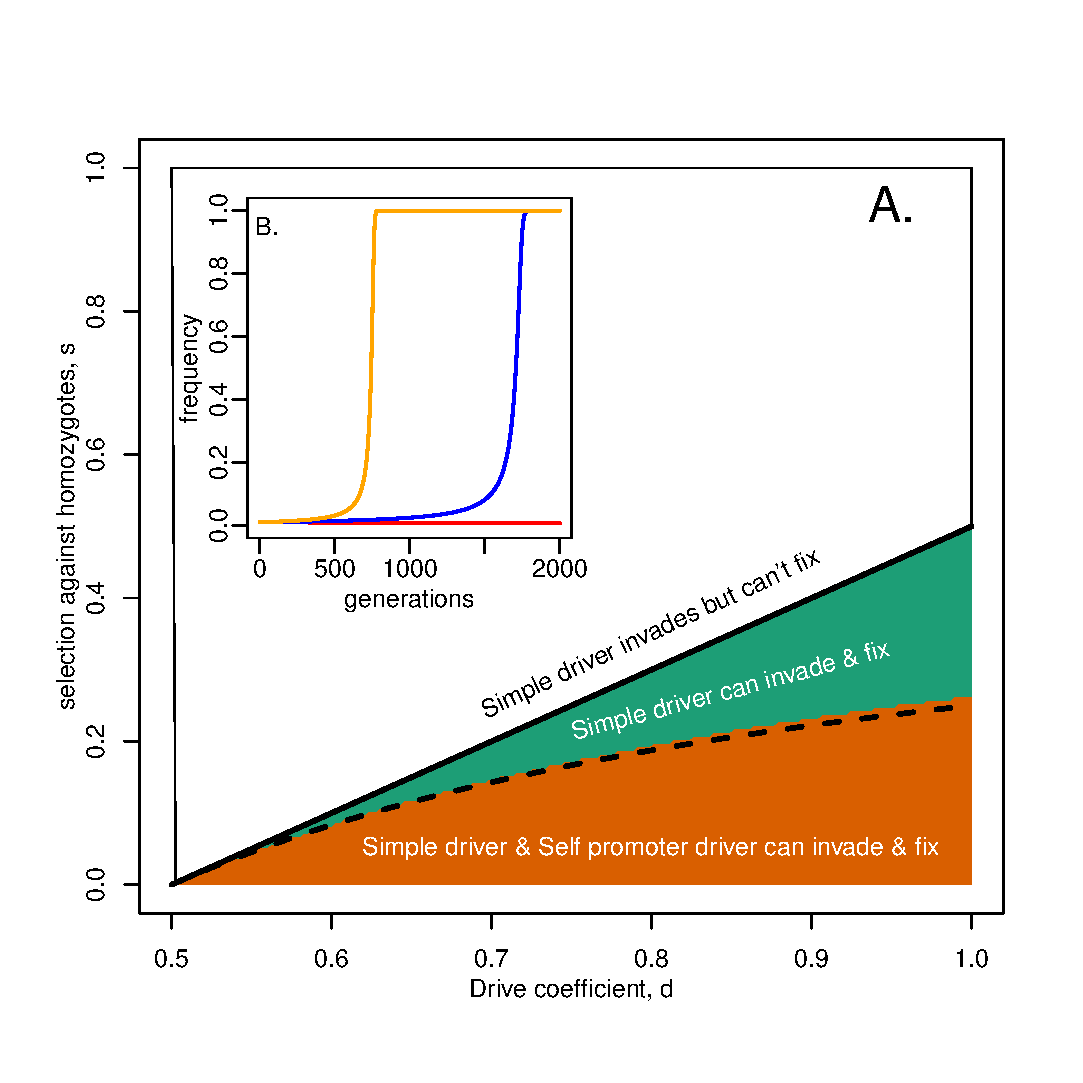
\includegraphics[width = 0.8 \textwidth]{Figures/invasion_space_recessive_driver.eps}
\caption{Invasion analysis for a female meiotic drive allele with
  recessive costs. First consider a simple female meiotic
  drive system, where the allele is transmitted a fraction $d>1/2$ of
  meioses in female heterozygotes, inspective
  of the allele carried by the fertilizing sperm. Such an allele can
  invade over all of the parameter space, and will be maintained as a
  protected polymorphism in the white region, and can fix in the
  population in all of the parameter space colored green,
  and will fix  or orange. Now consider an allele that is fairly transmitted through
  female meiosis when fertilized by a sperm carrying a different
  allele, but a fraction $d>1/2$ when a heterozygote egg is fertilized
  by a sperm carrying the allele (as depicted in Figure
  \ref{Eggsperm_2_allele_cartoon}). Such an allele can only invade in
  the region of parameter space colored orange, and it fixes over all
  of this parameter region. 
 In the inset we show trajectories of sperm-dependent female drive
 alleles that can invade the population, each allele has $s =0.1$ against the
 homozygotes and $d =0.6$, $0.7$, $0.8$ shown in yellow, blue, and red. 
 \gc{Likely make this Figure 1B.} } \label{Invasion_space}
\end{figure}


\subsection*{ sperm-egg haplotype balanced drive systems}

\begin{figure}
	\rotatebox{90}{\includegraphics[width = 0.8
          \textwidth]{Figures/Sperm_egg_cartoon_paper_Fig2.eps}}
\caption{Transmission probabilities righthand allele through female
  meiosis}  \label{Eggsperm_3_allele_cartoon}
\end{figure}


% \begin{figure}
% 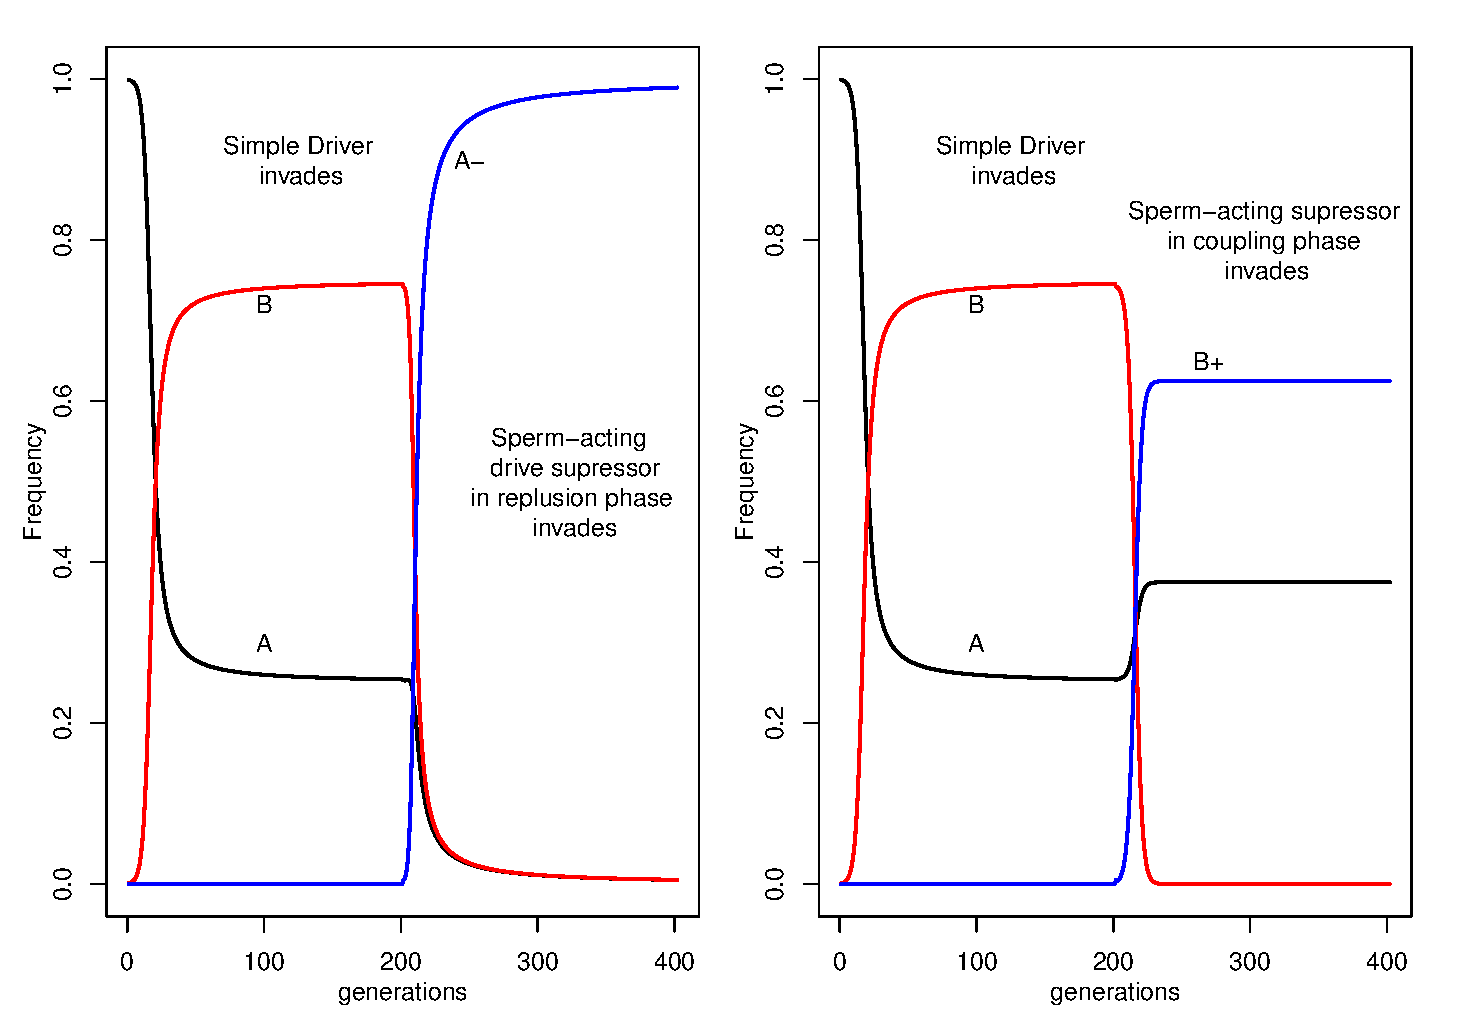
\includegraphics[width = 0.8 \textwidth]{Figures/trajectories_of_sperm_based_supressors.eps} 
% \caption{Trajectories of two sperm-based supressors of drive. Possibly
% merge this figure the 3 allele cartoon}  \label{Trajectories_of_supressors}
% \end{figure}



%%%%%%%%%%%%%%%%%%%%%%%%%
% TWO LOCUS MODEL [modify (general) / facilitate (helps ) / prevent (stops)] 
%%%%%%%%%%%%%%%%%%%%%%%%%
\yb{********* DO WE NEED TO DO THE MALE GENOTYPE THING HERE TOO? *********}

Above, we explored a model were a driver that drove in females when signaled by a complementary allele in sperm.  
We complement this single locus model of an allele with effects in
both male and with femalr, with  an alternative model of two linked loci - one female driver and the other a sperm allele which modifies the effect of drive upon fertilization. 
%Here, we examine an alternative scenario (and more realistic) in which
In this model initially a female meiotic driver, with no sperm-dependency, reaches drive-viability equilibrium (with two alleles
$A$ and $B$ are the ancestral non-driver and driver alleles).
Subsequently, a sperm-acting modifier of female meiotic drive arises tightly
        linked to this balanced locus (effectively creating a third
        allele/haplotype at this locus).
Assuming tight linkage between female driver and sperm modifier is consistent with the nature of well characterized meiotic drive systems 
	which are often maintained as polymorphic inversions with numerous linked modifiers (CITE).


\yb{??In the SUPP we explore the dynamics of a sperm modifier of female drive unlinked to the female driver??} 

%%%sperm-acting facilitator
We first consider a sperm-acting facilitator of
	female meiotic drive tightly linked to the $B$ background, 
	generating a third allele $B^{+}$ (i.e. the non-recombining haplotype of a
        driver allele and sperm-acting drive modifier). 
This new allele acts in sperm to increase the effectiveness of both
	the $B$ and  $B^{+}$ drive in $AB$ and $AB^{+}$ heterozygotes, see Figure \ref{Eggsperm_3_allele_cartoon} 
	for a simple schematic of this drive model.  
Naively, the $B^{+}$ may spread by capitalizing on the additional drive it causes; hover,  
	this is not the case for a few simple reasons. 
First, the sperm-acting drive facilitator (the novel $B^{+}$ haplotype) 
	arises when the ancestral driver ($B$) is at drive-selection balance, 
	and therefore immediately suffers a homozygous fitness cost.  
Worse yet, a novel $B^{+}$ haplotype most often helps 
	the $B$  allele drive ($B^+$ sperm meeting $AB$ eggs), because $B$ is initially more common than $B^{+}$. 
As $B^{+}$ facilitates $B$ these interactions frequently form 
	$BB^{+}$ heterozygotes that suffer the same fitness costs as $BB$. 
Therefore, sperm-acting drive facilitator alleles experience a profound disadvantage 
	in this scenario, even more so than under the previous two allele model. 
We have found no parameter range of this
	three allele system that allows the sperm-acting drive facilitator $B^{+}$ to
	invade the population. \yb{MATHS?}

%%%sperm-acting drive suppressors
While  sperm enhancement of a female drive cannot displace a polymorphic female driver, sperm based drive suppression - 
	that is sperm-acting alleles that act to restore  fairness of female meiosis can. 
If these sperm-acting drive suppressors arise on
	the non-driving $A$ background (creating a third allele $A^{-}$) ;
	or are unlinked to the drive locus they readily invade a population segregating
	for the drive system ($AB$, see Figure). 
This allele lowers the frequency of the original drive system (perhaps to zero),
	and spreads to fixation if it does not carry strong fitness costs
	(Figure \ref{Eggsperm_3_allele_cartoon} and \ref{Trajectories_of_supressors}A). 
This result is consistent with previous work showing that drive suppressors unlinked to, or in repulsion phase with drivers usually invade polymorphic drive systems \citep[e.g. ][]{Brandvain2012}.  

More surprisingly, sperm-acting suppressors of female drive can spread
	even when tightly linked to the original drive system (B), forming
	an novel third allele $B^{-}$ as above 
	(Figures \ref{Eggsperm_3_allele_cartoon} and \ref{Trajectories_of_supressors}B). 
$B^{-}$ displaces the original driver ($B$) by driving when not costly, 
	but by disrupting drive when transmitted to sperm it avoids low-fitness drive homozygotes ($BB^-$ and $B^-B^-$). 
Despite displacing the ancestral driver ($B$), self avoiding driver, $B^*$ it's equilibrium frequency is not always higher than that of $B$ \yb{(point to supp?)}. 

%\gc{Do we mention the In and Om locus here or in the discussion as a
%	 potential e.g. Do we mention the fact that the frequency of these
%	 newly invade sperm dodging alleles can be lower than the original system?}\\

\section*{Discussion}

Sexual reproduction is a high-stakes event that determines what gets transmitted to the next generation.  
As a consequence of this intense competition, alleles that gain a transmission advantage during reproduction 
	can succeed evolutionarily, even if they lower the 
        fitness of the population, 
	the mother whose offspring they will inhabit, 
	and even the organism in which they reside. 
This potential generates numerous conflicts  \cite{Burt2006} including sexual conflicts between mates \cite{Arnqvist2005}, 
	as well as conflicts between alleles that are overtransmitted in meiosis and the organisms they injure while doing so. 
Such conflicts and their resolution likely play a major role in the structure and evolution of many basic biological processes \citep{Rice2013}.

It seems that allowing sperm to influence the outcome of female meiosis would generate a confluence of these potential conflicts -- 
	sperm could actually assist an allele that distorts female meiosis.
However, this is not the case.
We find that an allele which acts through sperm to distort female meiosis in its favor %YB [too awkward / unclear?] 
	can rarely spread through a population if it bears any cost. 
Additionally, when this self-promoting driver can spread, it can only rarely 
	be maintained as a protected polymorphism, and due to its positive frequency dependence 
	it spends very little time at intermediate frequency.
As such, this type of exploitation cannot generate a sustained genetic conflict and so it is unlikely
	that female oogenesis and meiosis will evolve to prevent their effect.  
This likely explains why females can delay the completion of meiosis until after fertilization 
	without risking exploitation by collaborations by female
        drivers and sperm alleles.
%Male modification of recombination rates. \yb{trying to think through this \dots{}}

Why is it that an allele that biases female meiosis in its favor can generate a genetic conflict, but an allele in sperm that assists this female driver cannot? 
So long as the transmission advantage of female meiotic drive outweigh the organismal fitness cost to heterozygotes the female driver can spread when rare, and it increases in 		
	frequency until the fitness cost experienced when homozygous balances the transmission advantage.
By contrast a sperm promotor of female drive is only effective when matched with a heterozgyote female -- meaning that when rare this allele rarely enhances female drive. 
Even worse, when it does so it will preferentially find itself in a low fitness drive homozygote. 
Not only are drive-promoting sperm alleles unable to create a sustained genetic conflict, 
	but alleles in sperm with the opposite effect - that is those that prevent their own drive through female meiosis do maintain a polymorphisms and 
	provide evolution  with time and opportunity to further minimize drive.
This is because such drive suppressing alleles reduced their chances
of forming low fitness homozygotes. 
In fact, an allele in sperm which causes the alternate allele to drive can be favored (FIG), a counterintuitive result 
	consistent with the tenuous evidence that the non-driving
        $ln^-$ allele is over transmitted through female meiosis in $ln^-/ln^+$ heterozygote when fertilized by $ln^+$
        sperm \cite{agulnick, Pomiankowski1993}.   
More generally both linked and unlinked alleles may often spread that act through sperm to
reduce the opportunity of female meiotic drive in order to disable
segregating drive systems, by for example reducing the mechanistic
asymmetries that female drivers exploit. 


\gc{Is there some nice way to work in green beard ideas}


The interests of fertilizing sperm and female are quite well aligned during syngamy -- producing a viable and potentially fit offspring. 
%As noted above there are even opportunities for coevolution between sperm-based suppressors of female meiotic drive and the female genome.
Thus it seems plausible that aspects of oogenesis may actively evolve to facilitate the influence of sperm on ensuring a fair  outcome of female meiosis which generates fit offspring.
In light of that it is interesting to consider whether the phylogenetic variation in the stage of oogenesis when fertilization takes place reflects not
	only species' different reproductive ecologies, but also different selection pressures shaping the interaction of sperm alleles with female meioses. 
%\gc{Add short paragraph about sex chromosomes here? XY systems don't care. ZW systems (males ZZ, females ZW). If there is
%sex ratio distortion how could this play out?}


%\yb{DOES THIS GO ANYWHERE? }

% Males can potentially influence the outcome of meiosis even before fertilization. 
% For example in Drosophila and other taxa, sperm accessory
%         gland proteins (ACPs) increase the female recombination rate
%         \cite{SOMEthING}, and there is some evidence that there is
%         variance across male genotypes in there effect on female
%         recombination rate \cite{Stevison2012}.
% Presumably this is a pleiotropic consequence of the resolution of double strand breaks initiated by the stressful/toxic composition of ACPs. 
% However, a pleiotropic effect of this is to increase the recombination rate which can decrease the effectiveness of female meiotic drivers
% active during MI \citep{Brandvain}. 
% We speculate that other effects of sperm on female meiosis may also be tolerated by females as a way of ensuring meiotic fairness -- 
% 	that is females evolve to allow male influence on female meiosis in cases in which the male influence is  egalitarian. 



%Gametogenesis and meiosis are common times for genetic conflict. 
%This is a consequence of the fact that as the set of alleles that consitute
%	an individual are in the process of parting ways, 
%	with only a subset of them being assured transmission.
%In constrast, the perspective of the fertilizing sperm's genome is different, it has to live with the consequences of any distortion it causes 
%to female meiosis through the entire next life cycle of the organism. 
%It is therefore in the interest of the fertilizing sperm's genome to
%make a high fitness zygote even if that means alleles in sperm
%disrupting other copies of themselves from gaining a 
%transmission advantage through female meiosis.
  
\section*{Appendix}
In our first scenerio allele $A$ is the ancestral allele and allele
$B$ is our sperm dependent drive allele.
The sperm dependence of the drive is a form of assortative
transmission (mating), and so we have to keep track of the genotype frequencies.
Our genotype frequencies at birth are $x_{AA},~x_{AB},$ and
$x_{BB}$. These three genotypes have fitnesses $w_{AA},~w_{AB},$ and
$w_{BB}$, which are identical between males and females. As the
fitnesses are the same in males and females the frequencies of the
genotypes are identical in males and females, but in the following
equations they are marked with $\Mars$ and $\Venus$ respectively to
allow the reader to more easily follow the logic.
The frequency of the three genotypes at birth in the next generation is:
\begin{equation}
x'_{BB} =\frac{1}{\bar{w} } \Big( w_{BB} x_{BB}^{\Venus} (w_{BB} x_{BB}^{\Mars} +\frac{1}{2}
  w_{AB} x_{AB}^{\Mars} ) + w_{AB} x_{AB}^{\Venus} (d w_{BB}
  x_{BB}^{\Mars} +\frac{1}{2} d
w_{AB} x_{AB}^{\Mars} ) \Big),  \label{eqn.A1}
\end{equation}
\begin{equation}
x'_{AA} =\frac{1}{\bar{w} } \Big(  w_{AA} x_{AA}^{\Venus} (w_{AA} x_{AA}^{\Mars} + \frac{1}{2}
   w_{AB} x_{AB}^{\Mars}) + w_{AB} x_{AB}^{\Venus}(\frac{1}{2} w_{AA} x_{AA}^{\Mars}+ \frac{1}{2} 
  w_{AB} x_{AB}^{\Mars}) \Big),  \label{eqn.A2}
\end{equation}
and
\begin{eqnarray}
x'_{AB} = & \frac{1}{\bar{w} } \Big( w_{AA} x_{AA}^{\Venus}  ( w_{BB}  x_{BB}^{\Mars} + \frac{1}{2}
  w_{AB}  x_{AB}^{\Mars} ) +w_{BB} x_{BB}^{\Venus} ( w_{AA}  x_{AA}^{\Mars} + \frac{1}{2}
  w_{AB}  x_{AB}^{\Mars} )  \nonumber \\
& + x_{AB}^{\Venus}(\frac{1}{2}  w_{AA}  x_{AA}^{\Mars}+\frac{1}{2} (1-d)
 w_{AB}  x_{AB}^{\Mars} + \frac{1}{4}  w_{AB}
 x_{AB}^{\Mars} + (1-d)  w_{BB}  x_{BB}^{\Mars} ) \Big) \label{eqn.A3}
\end{eqnarray}
where the mean fitness of the population is
\begin{equation}
\bar{w} = w_{AA} x_{AA}+w_{AB}  x_{AB} +w_{BB}  x_{BB}.
\end{equation}


\bibliography{refs}

\section*{Supplementary Stuff}

\begin{figure}
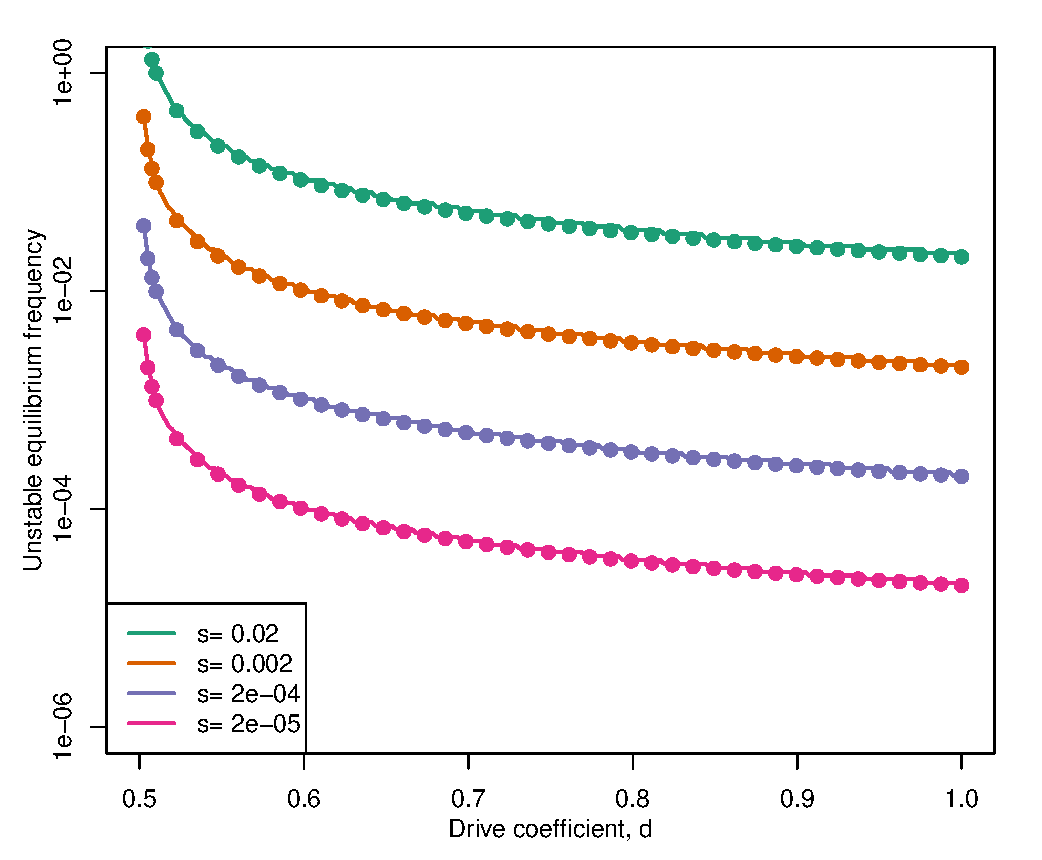
\includegraphics[width = 0.8 \textwidth]{Figures/bistable_x_vs_d_additive_s.eps} 
\caption{Bistable green-bearded allele when selection cost (s) acts
  additively, for an allele whose effect
 on female meoisis is mediated by sperm allele. }  \label{bistable_additive}
\end{figure}

\begin{figure}
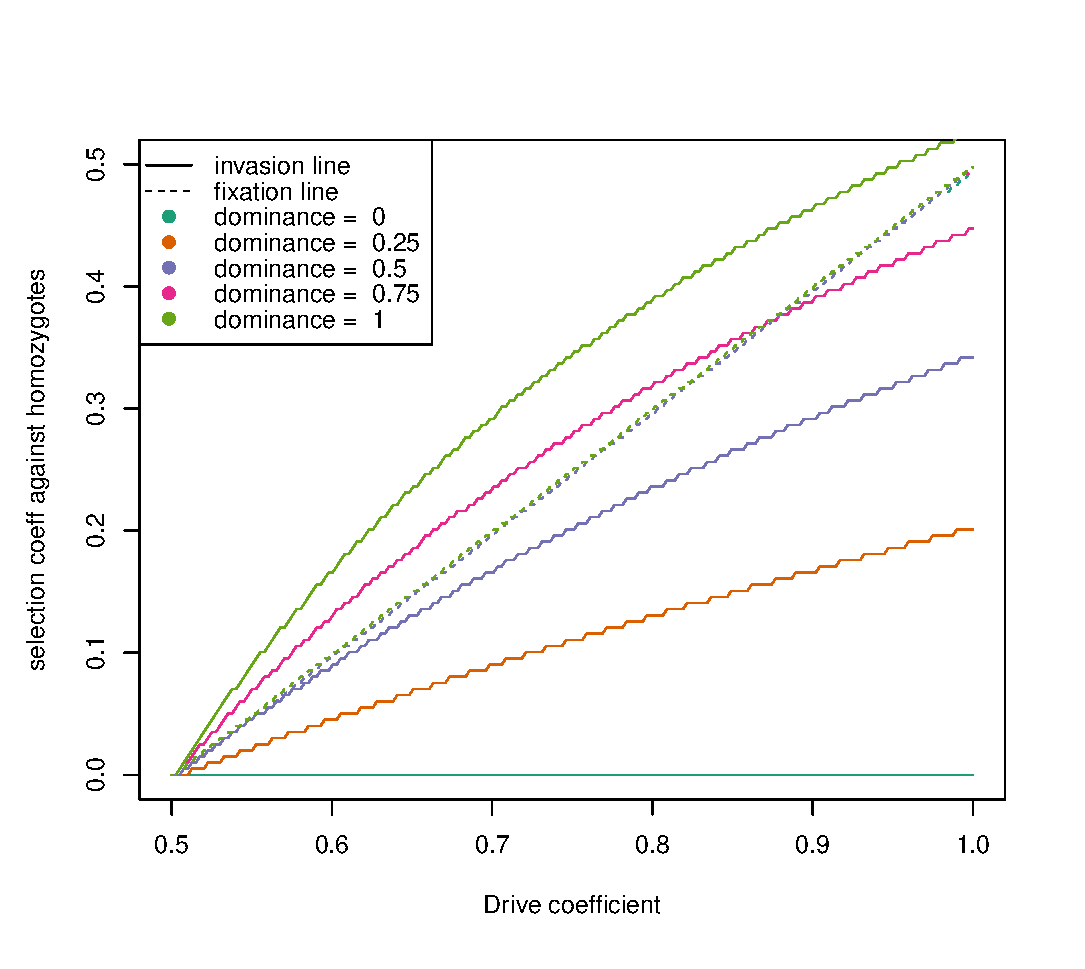
\includegraphics[width = 0.8 \textwidth]{Figures/effect_of_dominance_on_invasion_space_one_graph.eps} 
\caption{Invasion analysis of green-bearded sperm allele whose effect
 on female meoisis is mediated by the genotype of the fertilizing
 male. The area below the solid/dotted line is the parameter region
 where the allele can invade/fix (from $1/1000$ and $999/1000$
 \gc{maybe should lower this}). Note
 that all of the fixation lines are on top of each other as dominance
 parameter makes little difference here. The allele will be
 polymorphic in the parameter space where the solid (invasion) line
 falls above the dotted (fixation) line. Note that this is a very
 narrow parameter range, and only exists if the allele has a
 reasonable degree on dominance}  \label{Effect_of_dominance}
\end{figure}

\end{document}




\section*{OUTLINE}
\yb{YB: To me its (1) male enhancement of female drive cannot maintain a stable polymorphisms, and (2) An allele in sperm can evolve to suppress its drive in females.}
show that such alleles:
\begin{enumerate}
\item can't be balanced, \\
\item and homozygous problems are tested out at low freq.  \\
\item Any heterozygous problems, leads to a bistable allele\\
\item If these alleles take off they speed through to fixation\\
\item If allele has any drive ability in absence of sperm effect that is what allows it to enter the population
and sperm effect isn't a further cause of conflict. What if anything do we mean by this?\\
\item PERHAPS HERE WE INTRODUCE A SELF-RESTRAINING ALLELE
\end{enumerate}

Conclusion, such alleles are unlikely to cause evolution of female supressors, they test hemselves in a homozygous
state when they enter the population, and sweep quickly (all the way to fixation) if they enter the pop at all.\\


\begin{enumerate}
\item Setup a drive-selection balanced polymorphism in std. drive model. 
Do this by imagining the sperm-influence allele arising on the background of the driver, 
so the allele has drive capabilities, and can have had time to evolve new biology. 

Multilocus drivers held together with inversions, may offer a relatively large mutational/functional target.

Evolving on the new background means that the allele suffers the fitness consequences of the 
driver.  See A in Figure \ref{Eggsperm_3_allele_cartoon} \\
\item Sperm-based enhancers of drive can't invade (can they in some situations?). \\
\item Intuition is that the driver has already driven to a frequency 
where it is held in check by its cost in homozygotes. The sperm allele 
thus can't really help as it creates zygotes which suffer the homozygous fitness consequences.
\end{enumerate}

\subsection{So what can evolve?}
So what can happen?
\begin{enumerate}
\item Alleles that arise in linkage with drive systems, which when in sperm switch off drive, 
can spread. They benefit from drive, but avoid some of the
consequences ( (Bi) in Figure \ref{Eggsperm_3_allele_cartoon} ). Overall as a side product they are benefiting all in pop.\\
\item Presumably alleles that actually switch the allele that drives may do even better? As they'd end up in 
hets. Although they'd not drive, so hard to say. YB: There is evidence that In distorts meiosis in the other direction (they still drive when rare i.e. when not fused with drive supp sperm) \\
\item Alleles that cause sperm to switch off drive that arise on other background or unlinked to the drive system
are selected, and spread as fast as female supressors of drive ( (Bii) in Figure \ref{Eggsperm_3_allele_cartoon} )..\\
\item Alleles that in females facilitate the action of sperm supressors of drive (or vis versa) can spread. Haven't actually checked this.\\
\end{enumerate}

\section*{Conclusions.}